
\chapter{Présentation de l'unité d'accueil}
\label{chap:presentation_unite}

\section{Introduction}
\label{sec:intro_ch1}

L’Établissement Central de Rénovation du Matériel des Transmissions/1°RM (ECRMT), en tant qu’organe principal de la chaîne de soutien de l’Arme des Transmissions et des Systèmes d’Information, assure l’ensemble des missions assignées en termes de maintien en condition des moyens des transmissions en déploiement au sein des différentes structures de l’ANP. Dans ce chapitre, nous allons décrire l’organisation, les missions et les processus de production de l’établissement, avec un focus particulier sur le Département d’Assemblage des Moyens de Commutation et le Laboratoire Central de Recherche et Développement.

\section{Missions de l'ECRMT}
\label{sec:missions_ecrmt}

L’établissement est l’organe central du soutien technique des Transmissions au profit des forces, des unités et des structures du Ministère de la Défense Nationale. Il est chargé principalement des missions suivantes :

\paragraph{En termes de production}
\begin{itemize}
    \item L’assemblage des équipements, des parties d’équipements, sous-ensembles et accessoires des transmissions ou entrant dans la composition des équipements des transmissions et de guerre électronique.
\end{itemize}

\paragraph{Maintenance, Rénovation et Installation}
\begin{itemize}
    \item Rénovation des équipements de transmissions ;
    \item Maintenance du matériel des transmissions échelon 3° et 4° ;
    \item Le contrôle et l’évaluation techniques des moyens réalisés par la Direction Centrale des Transmissions et des Systèmes d’Information (DCTSI) ;
    \item La maintenance, l’administration et la supervision des réseaux de transmissions ;
    \item L’étude de faisabilité et l’installation des équipements de transmissions sur site et à bord des engins tactiques.
\end{itemize}

\paragraph{Développement, Formation et Veille technologique}
\begin{itemize}
    \item La formation spécialisée du personnel technicien sur les équipements de transmissions nouvellement acquis et l’organisation de stages pratiques ;
    \item L’établissement met au profit de la Direction Centrale des Transmissions des rapports de synthèse, d’analyse et de veille technologique ;
    \item L’établissement des audits internes des activités d’assemblage et de rénovation ;
    \item Assurer les coopérations, en termes de diffusion et de capitalisation des connaissances techniques, avec les différentes structures de Recherches et Développement.
\end{itemize}

\section{Structure Organisationnelle de l'ECRMT}
\label{sec:structure_ecrmt}

\begin{figure}[H]
    \centering
    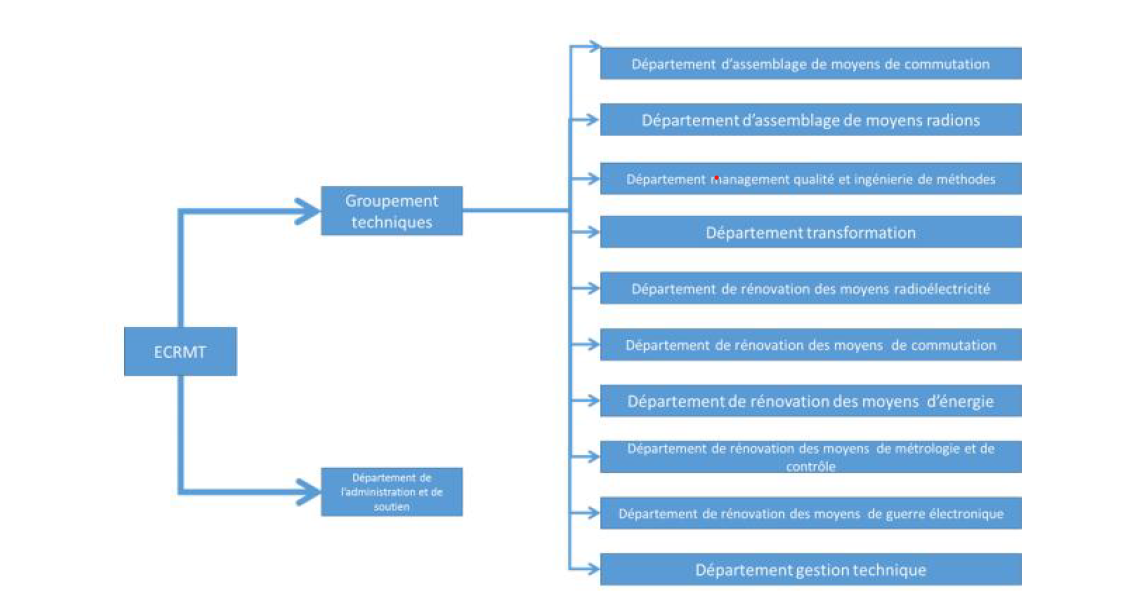
\includegraphics[width=0.9\textwidth]{./images/organigramme_ecrmt.png}
    \caption{Organigramme de la structure organisationnelle de l’ECRMT.}
    \label{fig:organigramme_ecrmt}
\end{figure}

\subsection{Département d'Assemblage des Moyens de Commutation}
\label{subsec:dept_assemblage}

Le Département d’Assemblage des Moyens de Commutation a pour mission la production des moyens de commutation. Son objectif stratégique est de gérer à terme la chaîne de montage de manière autonome, sans assistance étrangère, afin de maîtriser la production complète de tout équipement de transmissions.

\subsection{Processus d'assemblage}
\label{subsec:processus_assemblage}

Les processus d’assemblage sont organisés par zones, suivant le flux de production depuis la réception des composants jusqu’à la livraison du produit fini.

\paragraph{Magasin (Warehouse)}

\begin{figure}[H]
    \centering
     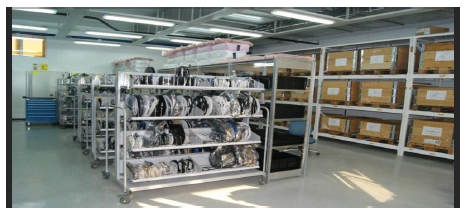
\includegraphics[width=0.8\textwidth]{./images/magasin.png}
    \caption{Vue du magasin (Warehouse) de l'ECRMT}
    \label{fig:magasin}
\end{figure}

Le processus d'assemblage débute au niveau du magasin par les étapes suivantes :
\begin{itemize}
    \item Réception et vérification des composants et consommables ;
    \item Enregistrement sur la base de données du système ERP ;
    \item Saisie des données de traçabilité (référence, date de fabrication, fabricant, etc.) pour chaque lot ;
    \item Préparation des kits de composants selon le plan de production.
\end{itemize}

\begin{figure}[H]
    \centering
     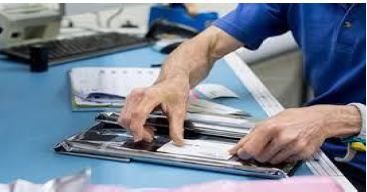
\includegraphics[width=0.8\textwidth]{./images/erp_interface.png}
    \caption{Interface du système de Gestion ERP utilisé à l'ECRMT}
    \label{fig:erp_interface}
\end{figure}

\textbf{Note :} La chaîne d'assemblage des moyens radio dispose d'un système de stockage automatisé avec 10 500 emplacements pour composants.

\begin{figure}[H]
    \centering
     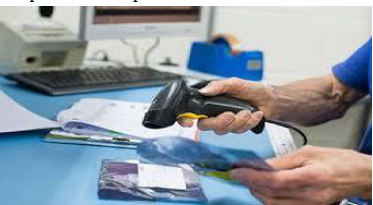
\includegraphics[width=0.8\textwidth]{./images/stockage_auto.png}
    \caption{Système de stockage automatisé de la chaîne d'assemblage des moyens radio}
    \label{fig:stockage_auto}
\end{figure}

\paragraph{Zone de production}

Cette zone comprend les lignes d'assemblage des cartes électroniques et les lignes d'assemblage final des produits.

\subsection{Lignes d'assemblage des cartes électroniques}
\label{subsec:lignes_electroniques}

Cette partie universelle de la chaîne d'assemblage se divise en deux types de lignes selon les composants utilisés.

\subsubsection*{Ligne d'assemblage SMT}

Dédiée à l'assemblage automatique des cartes électroniques à base de composants montés en surface (Surface Mount Technology).

\begin{figure}[H]
    \centering
    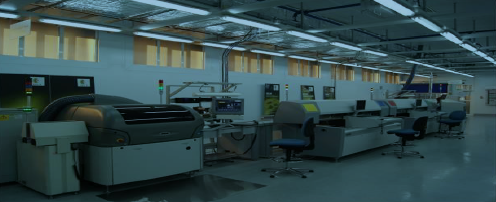
\includegraphics[width=0.8\textwidth]{./images/ligne_smt.png}
    \caption{Vue générale de la ligne d'assemblage SMT}
    \label{fig:ligne_smt}
\end{figure}

\textbf{Processus de la ligne SMT}

\begin{enumerate}
    \item \textbf{Sérigraphie :} Étendage automatique de la pâte à braser sur les circuits imprimés à l’aide de pochoirs (stencils) spécifiques.

    \begin{figure}[H]
        \centering
         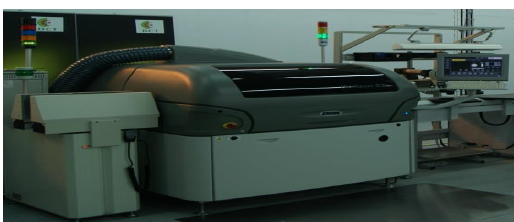
\includegraphics[width=0.6\textwidth]{./images/serigraphie.png}
        \caption{Machine de sérigraphie pour l’application de la pâte à braser}
        \label{fig:serigraphie}
    \end{figure}

    Ce processus est critique car il représente 60 à 70\% des erreurs de production.

    \item \textbf{Placement automatique des composants :} Positionnement précis des composants sur le circuit imprimé.

    \begin{figure}[H]
        \centering
         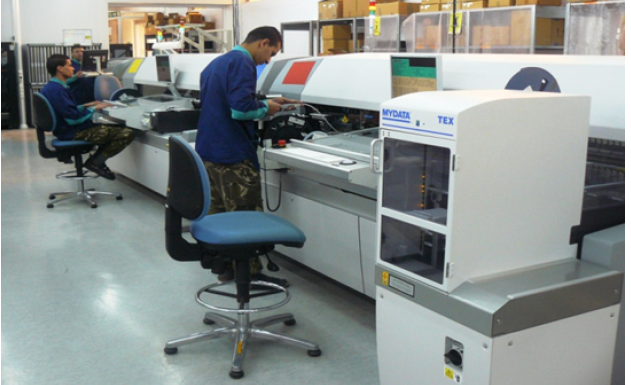
\includegraphics[width=0.6\textwidth]{./images/pick_and_place.png}
        \caption{Machine de placement automatique des composants (Pick \& Place)}
        \label{fig:pick_place}
    \end{figure}

    \textbf{Capacités des machines de placement :}
    \begin{itemize}
        \item Chaîne d'Assemblage des Moyens Radio : 90 000 composants/heure (3 machines $\times$ 30 000/heure)
        \item Chaîne d'Assemblage des Moyens de Commutation : 64 000 composants/heure (2 machines $\times$ 32 000/heure)
    \end{itemize}

    \item \textbf{Soudure par refusion :} Passage des cartes dans un four à refusion avec profils de température préprogrammés.

    \item \textbf{Inspection Optique Automatique (AOI) :} Vérification automatique de la présence, orientation et qualité des soudures.

    \item \textbf{Inspection par rayons X :} Contrôle des composants non visibles optiquement.

    \item \textbf{Inspection visuelle :} Contrôle complémentaire après sérigraphie et placement.
\end{enumerate}

\subsubsection*{Ligne d'assemblage THT}

Dédiée à l’assemblage manuel et semi-automatique des cartes à composants traversants (Through-Hole Technology).

\begin{figure}[H]
    \centering
     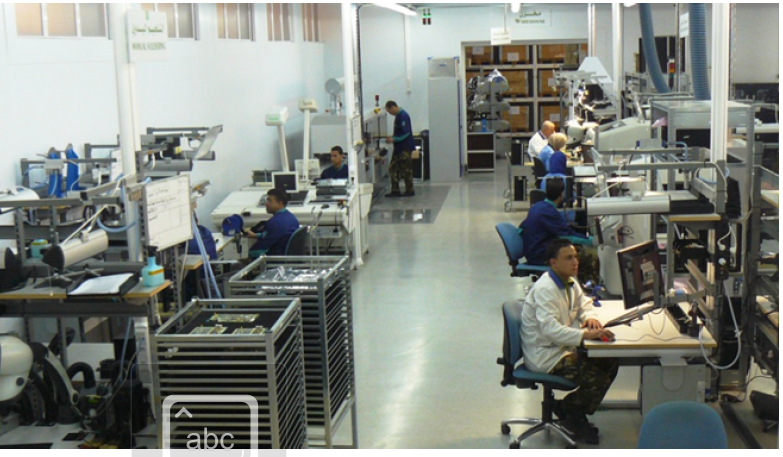
\includegraphics[width=0.8\textwidth]{./images/ligne_tht.png}
    \caption{Vue générale de la ligne d’assemblage THT}
    \label{fig:ligne_tht}
\end{figure}

\textbf{Processus de la ligne THT}

\begin{enumerate}
    \item \textbf{Préparation des composants (préformage) :} Coupe et mise en forme des pattes des composants.

    \item \textbf{Placement des composants :} Insertion manuelle ou semi-automatique des composants traversants.

    \begin{figure}[H]
        \centering
        \begin{minipage}{0.48\textwidth}
            \centering
             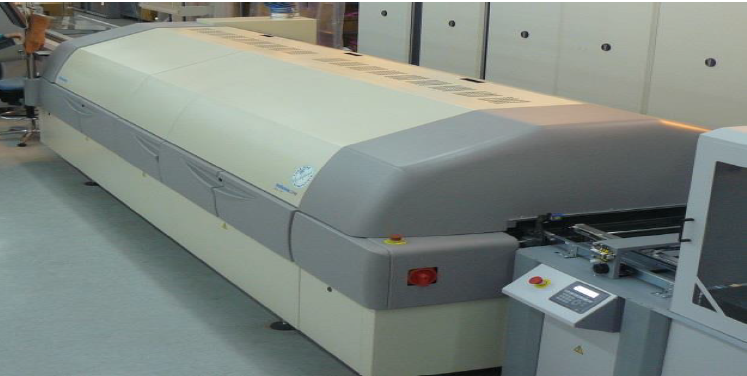
\includegraphics[width=\textwidth]{./images/placement_semi_auto.png}
            \caption{Placement semi-automatique des composants THT}
            \label{fig:placement_semi_auto}
        \end{minipage}\hfill
        \begin{minipage}{0.48\textwidth}
            \centering
            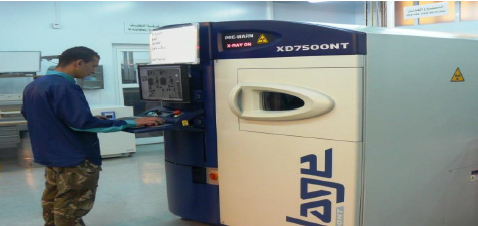
\includegraphics[width=\textwidth]{./images/placement_manuel.png}
            \caption{Placement manuel des composants THT}
            \label{fig:placement_manuel}
        \end{minipage}
    \end{figure}

    \item \textbf{Soudure des composants :} Réalisée par soudure sélective robotisée, soudure à la vague ou manuelle.

    \begin{figure}[H]
        \centering
         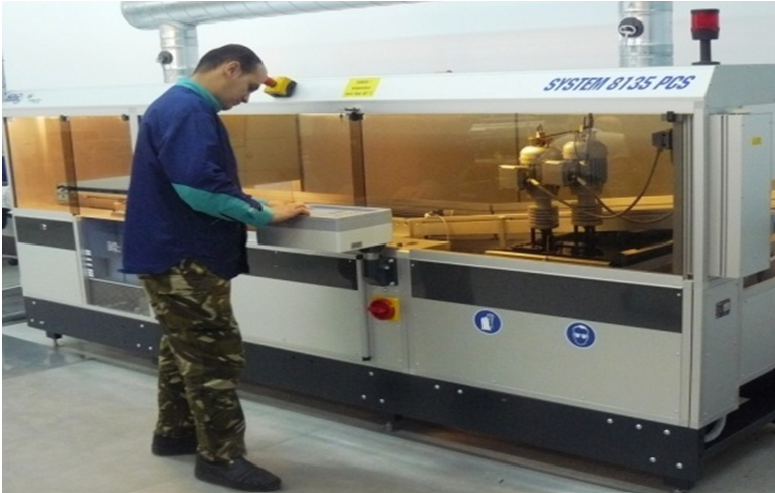
\includegraphics[width=0.7\textwidth]{./images/soudure_tht.png}
        \caption{Processus de soudure des composants THT}
        \label{fig:soudure_tht}
    \end{figure}

    \item \textbf{Inspection visuelle :} Contrôle qualité des joints de soudure.

    \begin{figure}[H]
        \centering
         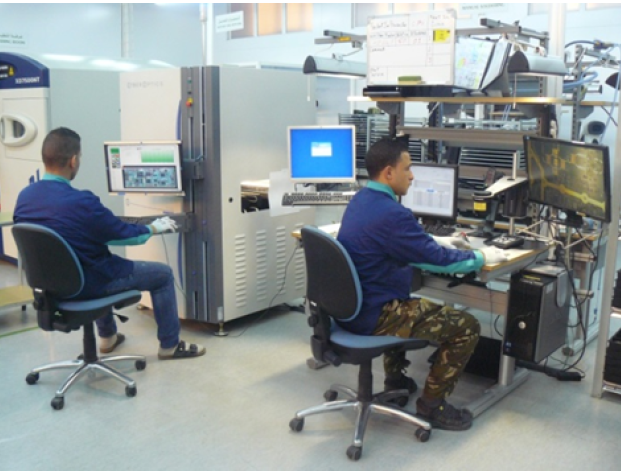
\includegraphics[width=0.8\textwidth]{./images/inspection_visuelle_tht.png}
        \caption{Exemples d'inspection visuelle des soudures THT}
        \label{fig:inspection_visuelle_tht}
    \end{figure}

    \item \textbf{Nettoyage des cartes :} Élimination des résidus chimiques (disponible sur la chaîne de commutation).

    \begin{figure}[H]
        \centering
         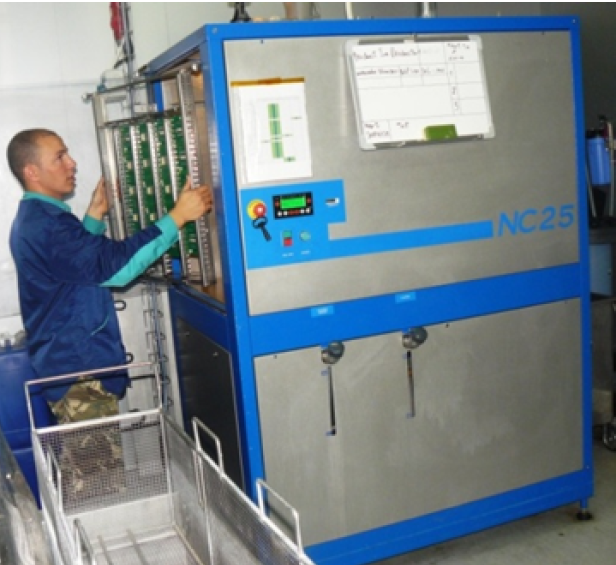
\includegraphics[width=0.6\textwidth]{./images/nettoyage_cartes.png}
        \caption{Station de nettoyage des cartes électroniques}
        \label{fig:nettoyage_cartes}
    \end{figure}

    Utilisation d'un mélange eau déminéralisée/alcool spécialisé.

    \item \textbf{Test des cartes :} Tests électriques, fonctionnels et chargement des logiciels.

    \begin{figure}[H]
        \centering
         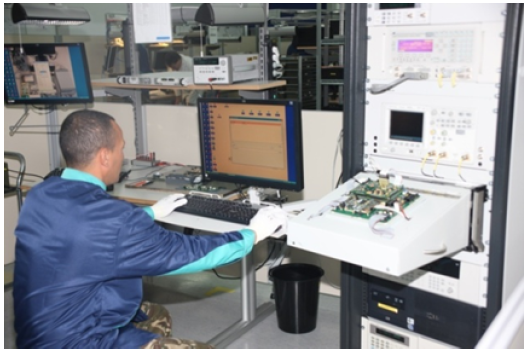
\includegraphics[width=0.6\textwidth]{./images/test_cartes.png}
        \caption{Station de test automatisé des cartes électroniques}
        \label{fig:test_cartes}
    \end{figure}
\end{enumerate}

\subsection{Lignes d'assemblage final}
\label{subsec:lignes_final}

\paragraph{Assemblage final}

Assemblage des différents sous-ensembles pour former les produits finis.

\begin{figure}[H]
    \centering
     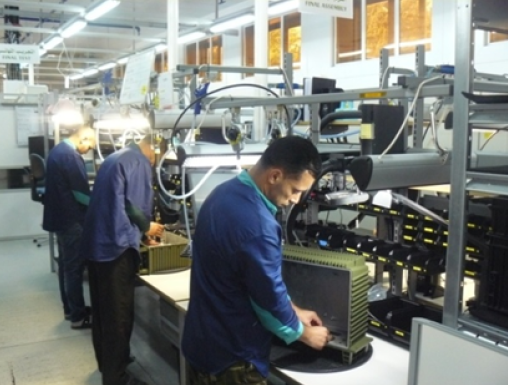
\includegraphics[width=0.8\textwidth]{./images/assemblage_final.png}
    \caption{Ligne d'assemblage final des produits}
    \label{fig:assemblage_final}
\end{figure}

\paragraph{Test final}

Tests conformes à la norme militaire MIL-STD-810 : fonctionnels, étanchéité, température, vibration.

\begin{figure}[H]
    \centering
    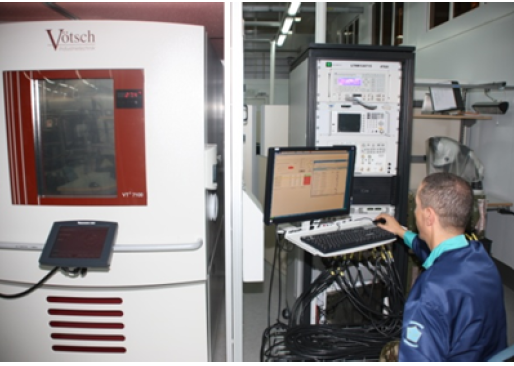
\includegraphics[width=0.8\textwidth]{./images/chambre_environnementale.png}
    \caption{Chambre de test environnemental pour les tests finaux}
    \label{fig:chambre_environnementale}
\end{figure}

\textbf{Exemple :} Le test de température de l'émetteur-récepteur RL532A dure 48 heures avec des cycles de -40°C à +55°C.

À l'issue des tests, les produits finis sont transférés au service logistique pour conditionnement et livraison aux Magasins Centraux.

\section{Qualité et Ingénierie}
\label{sec:qualite_ingenierie}

Les Départements d'Assemblage des Moyens Radio et de Commutation sont soutenus par le Département de Gestion de la Qualité et d'Ingénierie des Méthodes, chargé des missions suivantes :
\begin{itemize}
    \item Contrôle et assurance de la qualité ;
    \item Hygiène, Sécurité et Environnement (HSE) ;
    \item Audit interne ;
    \item Implémentation des nouveaux produits et configuration des machines ;
    \item Maintenance préventive et curative des moyens de production ;
    \item Amélioration et optimisation des processus d'assemblage ;
    \item Formation continue et certification des opérateurs.
\end{itemize}

\textbf{Note :} Le Département d'Assemblage des Moyens de Commutation est certifié ISO 9001 depuis septembre 2012.

\section{Laboratoire Central de Recherche et Développement}
\label{sec:labo_rd}

\subsection{Organisation du Laboratoire Central R\&D}
\label{subsec:org_labo}

Les fonctions de développement sont réparties en six spécialités principales :
\begin{itemize}
    \item Ingénierie des systèmes et intégration ;
    \item Développement logiciel (Software) ;
    \item Développement sur composants programmables ;
    \item Développement des circuits électroniques ;
    \item Développement mécanique ;
    \item Développement des stations de test.
\end{itemize}

Certains ingénieurs assument également des fonctions managériales :
\begin{itemize}
    \item Chef du Laboratoire Central R\&D ;
    \item Gestionnaire des projets de développement ;
    \item Gestionnaire de la documentation ;
    \item Responsable du matériel informatique (IT) ;
    \item Responsable de l'assurance qualité.
\end{itemize}

\begin{figure}[H]
    \centering
     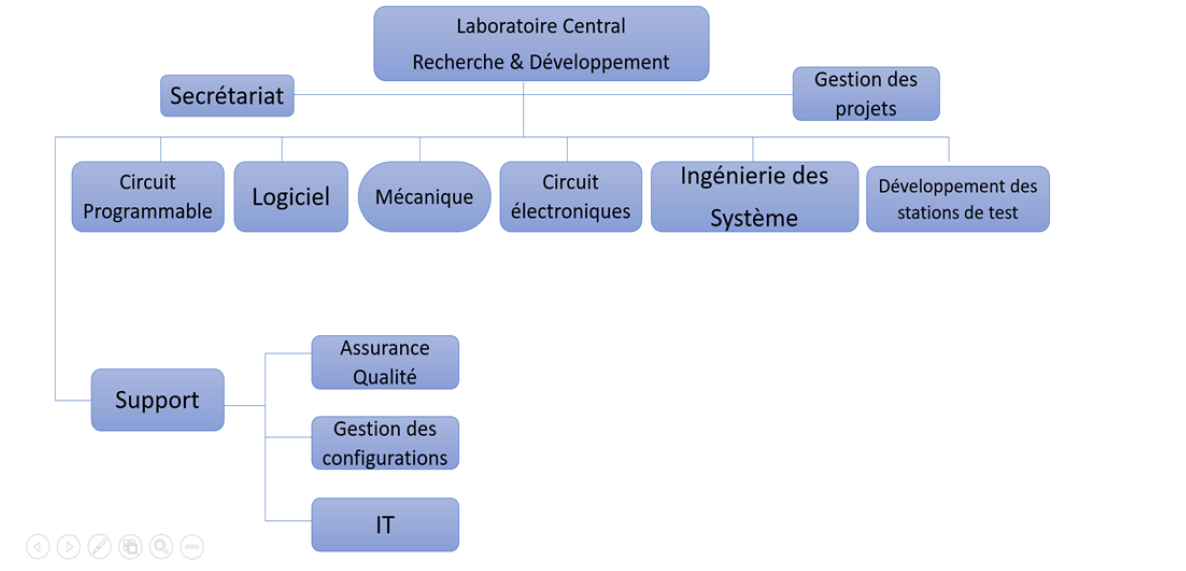
\includegraphics[width=0.9\textwidth]{./images/organigramme_rd.png}
    \caption{Organigramme fonctionnel du Laboratoire Central R\&D}
    \label{fig:organigramme_rd}
\end{figure}

\subsection{Missions et activités du Laboratoire Central R\&D}
\label{subsec:missions_labo}

Le Laboratoire Central R\&D a pour mission principale le développement, l'innovation et l'intégration de solutions technologiques avancées dans le domaine des systèmes de transmissions.

\paragraph{Activités techniques}
\begin{itemize}
    \item Développement de solutions innovantes pour les systèmes de transmissions de nouvelle génération ;
    \item Recherche et développement de solutions logicielles pour systèmes embarqués ;
    \item Modélisation et implémentation sur circuits programmables ;
    \item Conception électronique : choix d'architecture, schématisation, routage PCB ;
    \item Conception mécanique des produits et choix des matériaux ;
    \item Simulation des modèles (thermique, mécanique, etc.) ;
    \item Développement des processus et bancs de test ;
    \item Conception des interfaces de test.
\end{itemize}

\paragraph{Tâches managériales}
\begin{itemize}
    \item Gestion et planification des ressources de développement ;
    \item Analyse des risques et opportunités ;
\end{itemize}

\subsection{Infrastructure du Laboratoire Central R\&D}
\label{subsec:infra_labo}

Le Laboratoire Central R\&D s’étend sur 672 m² (48 m $\times$ 14 m) et comprend :
\begin{itemize}
    \item Quatorze (14) bureaux pour développeurs (répartis par spécialité) ;
    \item Bureau du gestionnaire des projets ;
    \item Bureau du chef de laboratoire ;
    \item Deux (02) centres de test (Hardware et Software) ;
    \item Deux (02) magasins (Hardware et Software) ;
    \item Salle de réunion ;
    \item Salle des machines ;
    \item Salle des serveurs ;
    \item Magasin pour matériel informatique ;
    \item Réception.
\end{itemize}

\subsection{Objectifs à long terme}
\label{subsec:objectifs_labo}

\begin{itemize}
    \item Augmenter le taux d’intégration dans la fabrication des équipements de transmissions ;
    \item Développer des compétences pour la conception de nouveaux équipements ;
    \item Renforcer les capacités en gestion de projets R\&D ;
    \item Concevoir des solutions adaptées aux besoins opérationnels, conformes aux normes internationales.
\end{itemize}


